\documentclass[a4paper,12pt]{article}
\usepackage[margin=0.75in]{geometry}
\usepackage{titlesec}
\usepackage{tocloft}
\usepackage{lmodern}
\usepackage{indentfirst}
\usepackage{fancyhdr}
\usepackage{setspace}
\usepackage[hidelinks,hypertexnames=false]{hyperref}
\usepackage{microtype}
\usepackage{graphicx}
\usepackage{float}
\usepackage{csvsimple}
\usepackage{booktabs}

\renewcommand{\thesection}{\arabic{section}}
\renewcommand{\thesubsection}{\thesection.\arabic{subsection}}

\renewcommand{\cftsecpresnum}{}
\renewcommand{\cftsecaftersnum}{: }
\settowidth{\cftsecnumwidth}{10: }
\renewcommand{\cftsubsecpresnum}{}
\renewcommand{\cftsubsecaftersnum}{: }
\settowidth{\cftsubsecnumwidth}{10.10: }
\setlength{\parindent}{30pt}
\setlength{\parskip}{0.3em}

\onehalfspacing

% Allow some stretch to reduce overfull \hbox warnings in long lines
\setlength{\emergencystretch}{2em}

\titleformat{\section}{\large\bfseries}{\thesection}{1em}{}
\titleformat{\subsection}{\normalsize\bfseries}{\thesubsection}{1em}{}

\begin{document}

% Avoid duplicate page anchors from title page
\pagenumbering{gobble}

\begin{titlepage}
    \centering
    \vspace*{3cm}
    {\Huge\bfseries Tensor Computation Benchmarks: \\ \texttt{Python} Vs. \texttt{NumPy} Vs. \texttt{PyTorch} Vs. \texttt{C} \par}
    \vspace{2cm}
    {\Large\textbf{Varak Tanashian} \par}
    \vspace{1.5cm}
    {\large Date: \today \par}
    \vfill
\end{titlepage}

% Resume normal page numbering after title page
\pagenumbering{arabic}
\setcounter{page}{1}

% ToC dynamically generated

\tableofcontents
\newpage

\section{Introduction}
\subsection{Overview}

In this project, I compare different tools for conducting common tensor computation operations. The focus is on evaluating their performance in terms of speed, memory usage, and ease of use. This is an important area of research as tensor computations are the backbone of many fundamental algorithms in machine learning and scientific computing. Understanding which tools to use (and why) will give the user both confidence and a deeper understanding of which tools to use. Even the most simple developments and innovations can lead to great leaps in performance as the effects of increased efficiency compound.

\subsection{Motivation}

Understanding performance differences across platforms is important for anyone who is working with high-throughput numerical workloads in their applications, whether in machine learning, scientific computing, or data analysis. By identifying the strengths and weaknesses of each tool, users can make informed decisions about which option is best suited to their needs. 

Typically, they have two options: they can either implement highly specialized, efficient algorithms tailored to their specific problems, or leverage pre-built, optimized libraries that provide these functionalities out of the box.

The trade-off centres on resource and time efficiency: building a computing engine in \texttt{C} demands significant effort, but widely used libraries like \texttt{NumPy} and \texttt{PyTorch} introduce considerable overhead and, being tied to interpreted languages, often run noticeably slower in practice. For any given large-scale application, this is a decision point that can affect not only computation speed but also the rate of development.

The choice of tool depends on the user's priorities. This project specifically focuses on raw compute-time efficiency: setting aside overhead and runtime environment considerations. As applications become more resource-intensive and advanced, the need for efficient computation becomes even more critical. The intention of this report is to provide a clear framework for when to make a tool from scratch and when to use a pre-built library.

\subsection{Objectives}
The main objectives are to objectively compare linear algebra performance across implementations in \texttt{Python}, \texttt{NumPy}, \texttt{PyTorch}, and \texttt{C}. In the concluding remarks, we will discuss the implications of the results and outline the key suggestions for users when choosing a tool for their specific needs.

\section{Background and Related Work}
\subsection{Historical Context}
Linear algebra has underpinned scientific computing for decades, with standardized kernels such as \textbf{BLAS} and \textbf{LAPACK} shaping expectations for performance and numerical stability. High-level ecosystems like \texttt{Python} made these capabilities accessible through libraries that delegate heavy computations to optimized native code. This way, developers could focus on high-level logic and technological innovations rather than the calculations that happen in the background. \texttt{NumPy} established a consistent array model with vectorized primitives that map cleanly onto \textbf{BLAS} backends. \texttt{PyTorch} expanded the model with automatic differentiation and optional \texttt{GPU} acceleration while retaining efficient tensor kernels. This project situates itself in that lineage by comparing practical throughput across plain \texttt{Python}, \texttt{NumPy}, \texttt{PyTorch}, and a purpose-built \texttt{C} baseline for common operations.

\subsection{Related Studies}
Prior benchmarks often assess individual operations or focus on single frameworks under fixed hardware and library configurations. Studies that compare compiled and interpreted stacks typically emphasize the cost of dispatch, data layout, and memory bandwidth rather than pure arithmetic. \texttt{GPU}-focused work highlights the trade-off between kernel launch overhead and arithmetic intensity, where small problems favor \texttt{CPUs} and larger problems favor \texttt{GPUs}. End-to-end \texttt{ML} benchmarks are informative but can obscure microkernel behavior due to preprocessing and I/O effects. This work narrows scope to core tensor arithmetic so differences reflect implementation choices rather than pipeline factors.

\subsection{Research Gap}
Existing comparisons rarely unify the parsing of test cases, batched execution, and standardized \texttt{JSON} reporting across heterogeneous implementations. They also tend to under-document the mechanics that affect timing repeatability, such as warmups, log-scale visualization, and skipping pathological sizes for naive kernels. Moreover, practical users need guidance that maps problem size and operation type to a suitable tool without overfitting to one machine. This report addresses those gaps by using a single bench-file format and a common runner that enforces comparable timing semantics. The result is a portable harness that favours clarity and reproducibility over benchmark maximalism.

\section{System Design and Architecture}
\subsection{Architecture Overview}
The system centers on a \texttt{Python} orchestrator that compiles and invokes all implementations in a single batch, then aggregates results into a \texttt{JSON} report. A shared bench-file format specifies operations, shapes, and data using simple tags so each implementation can parse identically. For each implementation, a \texttt{JSON} object per test with shapes, run counts, and timing statistics is produced. This will be used later on for analysis. A visualization script then groups results by operation and shape, generating bar charts, box plots, and tables on a log scale. This separation of orchestration, execution, and reporting keeps the code modular and easy to extend. Future tests can easily expand on this report by adding more modules (testing more libraries), creating new tests, and refining existing ones.

\subsection{Core Components}
The orchestrator compiles the \texttt{C} binary if needed, discovers tests, filters oversized cases, and runs each implementation with consistent environment variables. The \texttt{C}, \texttt{NumPy}, \texttt{PyTorch}, and \texttt{Vanilla Python} backends each provide a bench mode that parses the bench file and emits structured timing data. The bench parser supports scalar-fill after the \texttt{DATA} tag, allowing concise definitions of large constant tensors. The plotting module creates visualizations for all cases and aggregates a table with all of the results.

\subsection{Data Flow}
Benchmark blocks are read from a text file and split into independent cases by the runner. Each backend parses the same tokens into in-memory tensors, executes warmups, and then times a fixed number of runs per case. The backends emit \texttt{JSON} lines to stdout, which the runner collects and writes to a consolidated report file. The visualization tool loads this report, groups rows by operation and shape, and renders charts plus tabular summaries to the results directory. This linear flow avoids intermediate mutable state and makes failures localized and easy to diagnose.

\section{Implementation Details}
\subsection{Code Structure}
The codebase is organized by implementation, with separate entry points for \texttt{C}, \texttt{NumPy}, \texttt{PyTorch}, and \texttt{Vanilla Python}. The runner script provides build orchestration, environment detection for \texttt{Python} interpreters, and process management with timeouts. Bench parsing logic is duplicated across backends to ensure consistent semantics for shapes, data, and scalar parameters. All backends share the same operation set: element-wise add, matrix multiply, batched matrix multiply, scalar multiply, and dot product. Each backend returns a consistent \texttt{JSON} schema so the plotting stage can remain implementation-agnostic. A part of the motivation behind the "vanilla" implementations is to show that even unoptimized hand-written custom engines are very competitive for small and medium problems, and sometimes even faster. 

\subsection{Libraries Used}
The \texttt{C} implementation uses the \texttt{C99 standard library} and a simple timer for portability, prioritizing minimal dependencies. \texttt{NumPy} and \texttt{PyTorch} rely on their native tensor engines, which can leverage multi-threaded \textbf{BLAS} and, for \texttt{PyTorch}, optional \textbf{CUDA} acceleration. The Vanilla \texttt{Python} version uses nested lists and straightforward loops to make algorithmic costs explicit. \texttt{Matplotlib} and \texttt{NumPy} are used in the visualization pipeline to render log-scale charts and compute basic statistics. The entire workflow is driven by standard \texttt{Python} tooling for portability across platforms.

\subsection{Testing}
Small illustrative examples in each backend print intermediate results to validate shape handling and arithmetic behaviour. The bench mode focuses on timing and does not perform cross-implementation numerical comparisons during batch runs. Correctness is encouraged by shared input definitions and by using simple, deterministic test values in the bench file. Users can extend the harness with explicit correctness checks when needed, trading off additional overhead for verification. In practice, the primary goal here is consistent timing under a fixed input specification.

\section{Benchmarking Methodology}
\subsection{Experimental Setup}
The runner enforces consistent timing parameters via environment variables for runs and warmups, and it executes all tests in one process per implementation. By default, it compiles the \texttt{C} binary with \texttt{-O2} and enables skipping of computationally expensive or oversized cases for \texttt{C} and \texttt{Vanilla Python}. The \texttt{Python} interpreter can be selected from a local virtual environment to stabilize library versions. GPU timing in \texttt{PyTorch} includes synchronization to ensure that recorded durations reflect completed work. Hardware specifics are not recorded automatically, so results should be interpreted relative to the host system.

\subsection{Measurement Techniques}
All \texttt{Python} backends use \texttt{time.perf\_counter()} and the \texttt{C} backend uses \texttt{clock()} to measure elapsed time. Each case runs a configurable number of warmups to amortize initialization effects before recording timed iterations. Per-case statistics include the median, mean, population standard deviation, and the raw list of trial times for box plots. Visualization uses log-scale axes with decade ticks to compare a wide range of magnitudes cleanly. Only execution time is measured; memory and utilization metrics are out of scope for this version.

\subsection{Data Analysis}
After execution, the runner writes a single \texttt{JSON} report consolidating all implementations and test cases. The analysis script groups rows by operation and the pair of operand shapes to enable side-by-side comparisons. Bar charts display medians across implementations, while box plots show variation when multiple timings are available. An aggregate table is generated in both \texttt{CSV} and \texttt{Markdown} formats, substituting “skipped” when a backend omits a case. Outputs are written under a versioned results directory for easy inspection and sharing.

\section{Results and Analysis}
\subsection{Performance Metrics}
The primary metric is median execution time per case because it is robust to occasional outliers. Mean and standard deviation provide context for variability across runs and can flag unstable scenarios. Box plots visualize the distribution of raw timings on a log scale to surface skew and spread. Results are reported per operation and shape, allowing fair comparisons across backends on identical inputs. Skipped entries are retained in tables so readers can see which sizes are intentionally filtered by policy.

\subsection{Comparative Analysis}
Comparisons are made within each operation class to keep semantics consistent across implementations. Element-wise addition and dot products are typically latency-bound and favor low-overhead paths on small inputs. Matrix multiplications benefit from optimized kernels and threading in \texttt{NumPy} and \texttt{PyTorch}, particularly at larger sizes. Batched matrix multiplication amplifies these trends by increasing arithmetic intensity relative to dispatch overhead. The \texttt{C} implementation provides a transparent baseline for algorithmic cost, while \texttt{Python} list code clarifies the impact of interpreter overhead.

\subsection{Key Findings}
On small problems, the lowest-overhead path often wins, making the \texttt{C} and Vanilla \texttt{Python} implementations competitive for simple operations. 

\begin{figure}[H]
  \centering
  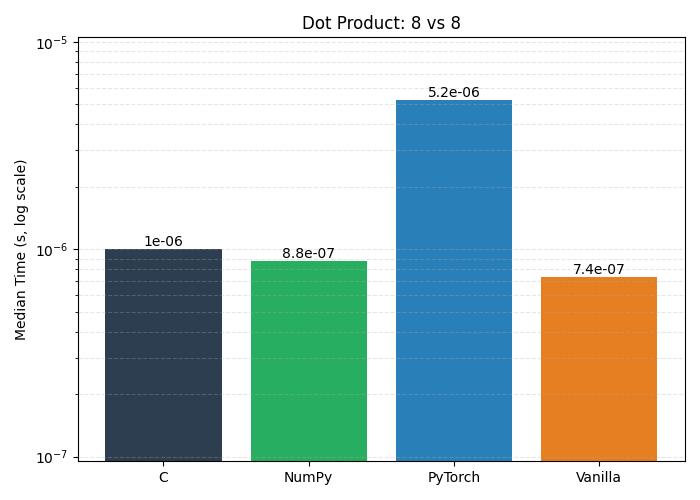
\includegraphics[width=0.7\linewidth]{results/bar/DOT_8_8.png}
  \caption{Results of a simple dot product operation.}
  \label{fig:one}
\end{figure}

As we approach medium-sized problems of low complexity, the vanilla \texttt{Python} implementation quickly starts to lag behind, while the \texttt{C} implementation remains ahead of the pack.

\begin{figure}[H]
  \centering
  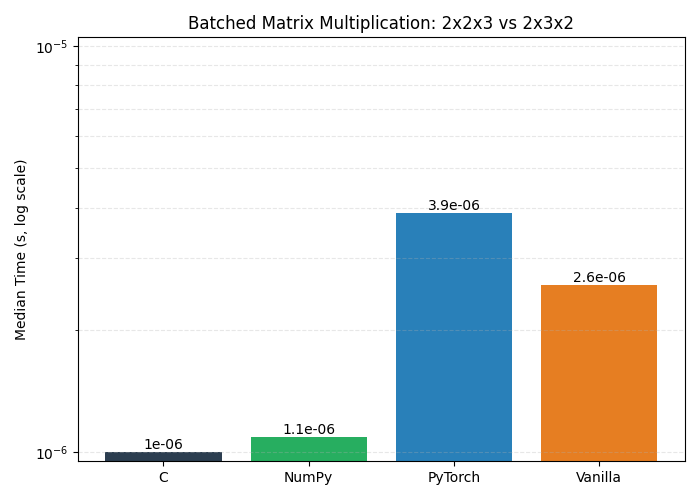
\includegraphics[width=0.7\linewidth]{results/bar/BMM_2x2x3_2x3x2.png}
  \caption{Results of 3D tensor multiplication.}
  \label{fig:two}
\end{figure}

Notice how \texttt{PyTorch} lags behind significantly, as it is not optimized for small workloads nor specifically designed for computation. As problem sizes increase, the overhead of \texttt{PyTorch} becomes less significant, and it starts to catch up with \texttt{NumPy}.

Problem sizes grow further, and vectorized libraries close the gap and then exceed naive baselines due to tuned kernels and better cache behavior. For large matrix multiplications, optimized backends routinely outperform unoptimized loops by orders of magnitude. \texttt{PyTorch} can benefit from \texttt{GPU} acceleration when available, but launch overhead dominates at tiny sizes. These patterns are consistent with the aggregate tables and per-case plots generated by the harness.

\begin{figure}[H]
  \centering
  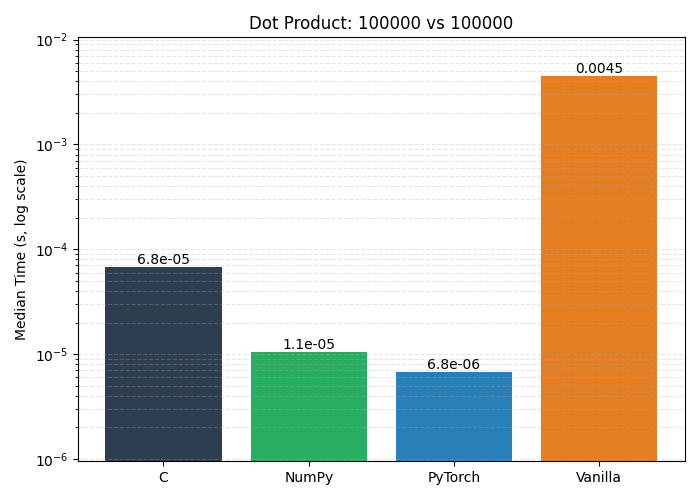
\includegraphics[width=0.7\linewidth]{results/bar/DOT_100000_100000.png}
  \caption{Dot product of 100{,}000-dimensional vectors.}
  \label{fig:three}
\end{figure}

Eventually, the operations become so large that the optimizations made by \texttt{NumPy} and \texttt{PyTorch} start to pay off, and they begin to outperform the \texttt{C} implementation as well.

\begin{figure}[H]
  \centering
  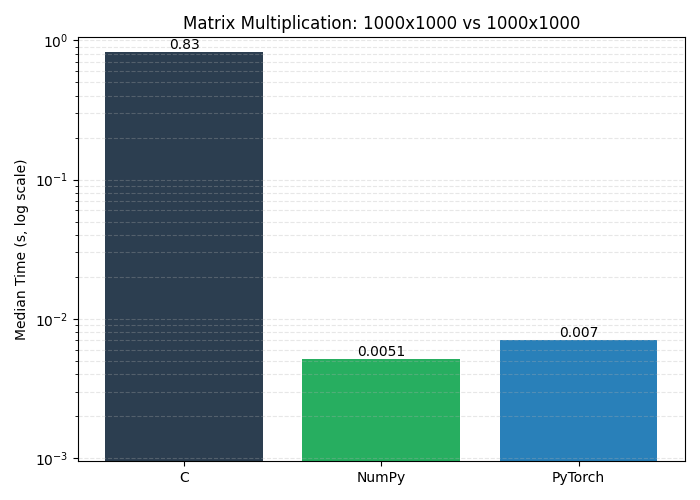
\includegraphics[width=0.7\linewidth]{results/bar/MM_1000x1000_1000x1000.png}
  \caption{Matrix Multiplication of 1000x1000 matrices.}
  \label{fig:four}
\end{figure}

Soon enough, the difference becomes so drastic that it is not even worth
measuring the \texttt{C} and Vanilla \texttt{Python} implementations, as they
are so far behind that they are not even competitive. \texttt{NumPy} and \texttt{PyTorch} finish in milliseconds, while \texttt{C} and Vanilla \texttt{Python} take entire minutes.

\begin{figure}[H]
  \centering
  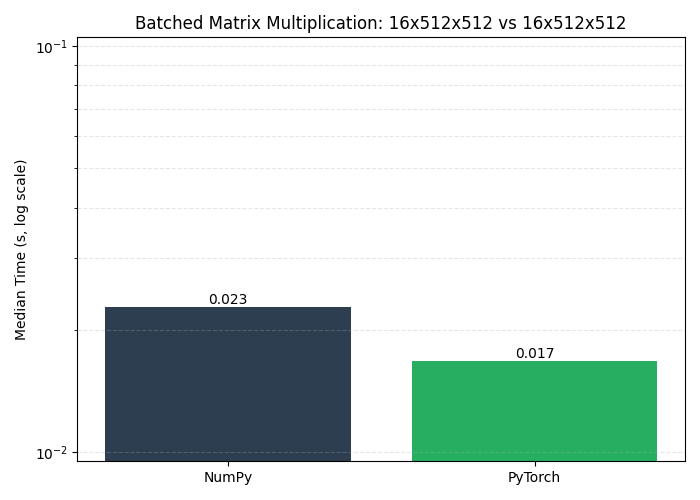
\includegraphics[width=0.7\linewidth]{results/bar/BMM_16x512x512_16x512x512.png}
  \caption{Batched matrix multiplication for tensors of shape 16x512x512.}
  \label{fig:five}
\end{figure}

\subsection{Aggregate Performance Results}

To provide a comprehensive overview of the performance characteristics across all implementations and test cases, Table~\ref{tab:aggregate} presents the median execution times for each operation type and tensor shape combination. The table includes results from all four implementations: \texttt{C}, \texttt{NumPy}, \texttt{PyTorch}, and Vanilla \texttt{Python}.

The timing values are reported in seconds, with scientific notation used for very small values. Entries marked as "skipped" indicate cases where the implementation was intentionally excluded from testing, typically due to computational infeasibility for the Vanilla \texttt{Python} implementation on large problems.

This aggregate view complements the individual visualizations by allowing direct comparison across all implementations for each specific operation and shape combination. The data clearly demonstrates the performance trade-offs between different approaches, with optimized libraries like \texttt{NumPy} and \texttt{PyTorch} showing significant advantages for larger computations, while low-overhead implementations like \texttt{C} excel at smaller scales.

\begin{table}[H]
\centering
\small
\label{tab:aggregate}
\begin{tabular}{@{}lllrrrl@{}}
    \textbf{Operation}* & \textbf{Shape A} & \textbf{Shape B} & \textbf{C} & \textbf{NumPy} & \textbf{PyTorch} & \textbf{Vanilla} \\
  \midrule
\csvreader[
  separator=comma,
  head to column names,
  late after line=\\,
  late after last line=\\\bottomrule
]{results/table/aggregate_table.csv}{
  Op=\Op,
  {Shape A}=\ShapeA,
  {Shape B}=\ShapeB,
  C=\C,
  NumPy=\NumPy,
  PyTorch=\PyTorch,
  Vanilla=\Vanilla
}{
  \Op & \ShapeA & \ShapeB & \C & \NumPy & \PyTorch & \Vanilla
}
\end{tabular}
\caption{Aggregate performance results across all implementations and test cases. Times are reported in seconds using median execution time. "Skipped" entries indicate computationally infeasible cases.}

\begin{small}
	*\textit{Acronyms}: \hspace{0.5cm}
	\textbf{ADD} = Addition, \hspace{0.5cm} \textbf{MM} = Matrix Multiply, \hspace{0.5cm} \textbf{SCAL} = Scalar Multiply, \hspace{0.5cm} \\ \textbf{DOT} = Dot Product, \hspace{0.5cm} \textbf{BMM} = Batched Matrix Multiply.
\end{small}

\end{table}

\section{Discussion}
\subsection{Interpretation of Results}
From these results, we understand the importance of using the correct tool for the correct workload. Small, frequent operations benefit from lower-level or lower-overhead paths, especially pre-compiled ones like those in \texttt{C}. As the computations get larger, they start to justify library dispatch costs. Warmups and batched execution materially improve timing stability and should be retained for reproducibility. Skipping extreme cases in \texttt{C} and Vanilla \texttt{Python} keeps total runtime reasonable without obscuring trends. Practitioners should calibrate thresholds and runs to their own machines for decision-grade comparisons. Given the magnitude of the differences and the sample sizes used for running these tests, it would be reasonable to expect similar trends in other environments.

\subsection{Limitations}
The current setup does not collect memory usage, hardware counters, or threading details, which limits multi-factor analysis. Library backends and \textbf{BLAS} configurations may differ across systems, which would introduce variability not controlled by the runner. The \texttt{C} timer’s granularity and OS scheduling can affect microsecond-scale measurements, especially on very fast kernels. GPU availability and configuration are environment-dependent and may change the relative standings.

\subsection{Implications}
Given the constraints, one should take these results as indicative of clear trends rather than exact measures of performance. Small, simple, and highly repeated tasks benefit from custom (even un-optimized) pre-compiled implementations, while heavier, deeper computations require sophisticated approaches like those found in \texttt{NumPy} or \texttt{PyTorch}. If decisions hinge on narrow margins, teams should supplement timings with correctness checks and environment capture to make a decision. For production, the decisive factors include maintainability, deployment constraints, and library availability, not just raw speed.

\section{Conclusion and Future Work}
\subsection{Summary}
This work presents a unified, practical framework for benchmarking core tensor operations across \texttt{C}, \texttt{NumPy}, \texttt{PyTorch}, and Vanilla \texttt{Python}. A shared bench format, consistent timing semantics, and standardized \texttt{JSON} reporting enable clear comparisons. Visualizations on log scales and aggregate tables make large performance differences readable at a glance. The results align with expectations: low-overhead paths excel on small tasks, while optimized libraries dominate large matrix operations. The system favors reproducibility and clarity so users can make grounded, context-specific choices.

\subsection{Future Directions}
Potential future improvements could add correctness checks, hardware metadata capture, and optional memory profiling to enrich context. Extending the operation set to include convolutions, reductions, inverses, and sparse primitives would also be a good idea. Parallel and distributed variants could measure scaling properties beyond single-process runs. A \texttt{CUDA}-backed \texttt{C} path or bindings to vendor libraries would enable deeper GPU comparisons. Finally, a configuration file for thresholds and environment settings would make the harness easier to tune and share.

\end{document}
